\documentclass[../../layout.tex]{subfiles}

\begin{document}
\chapter{Método}
Para demonstrar como foi desenvolvido o material técnico e a aplicação de valor deste projeto, seguimos por diversas pesquisas e análises de como chegar à um desenvolvimento onde fosse viável sua execução, aplicação e escalabilidade, para que tenha necessidade futura de seu uso contínuo.

\section{Levantamento Bibliográfico}
A aplicação do projeto de forma adequada, levou à muitas buscas teóricas e estudos variados da maneira que pode ser avaliada e aplicada às diversas tecnologias e ferramentas.\par
Dentre elas, podemos citar as mais importantes considerações levadas:

\begin{enumerate}[label=\alph*)]
\itemsep0em
	\item levantamento de requisitos;
	\item linguagem de programação;
	\item ferramentas tenológicas para auxiliar o desenvolvimento e organização do projeto;
	\item casos de uso;
	\item aplicações reais com objetivos similares;
	\item aplicações com as mesmas \emph{frameworks} utilizadas no projeto;
	\item viabilidade.
\end{enumerate}

\subsection{Levantamento de Requisitos}
Foco em analisar quais objetivos queremos chegar e por qual método iremos realizar isso. Utilizamos o microprocessador Raspberry pela sua facilidade de acesso e quantidade de informações de diversos usuários e desenvolvedores, para controlar dispositivos pela internet através de uma maneira simples e otimizada via celular ou computador.

\subsection{Linguagem de Programação}
Como existem diversas linguagens de programação, foram realizadas análises variadas das mesmas para entender qual o melhor uso e como se encaixam à essa aplicação que escolhemos. Dentre as muitas, optamos por selecionar linguagens que possuem boa interação com o \emph{front-end} e o \emph{back-end}, mantendo um bom desempenho e com um visual prático para o desenvolvimento.

\subsection{Ferramentas Tenológicas}
Ferramentas são necessárias para auxiliar no desenvolvimento, sejam anotações em um tablet, dispositivos auxiliares para realizar análises ou medições, que não fazem parte exatamente do projeto final, mas tem um grande envolvimento com o mesmo.

\subsection{Casos de Uso}
Empresas focam em atender a necessidade de seus clientes de uma forma em que eles saiam satisfeitos e recomendem o serviço, produto ou suporte. Isso faz com que muitas soluções sejam críticamente pensadas e desenvolvidas. Para validação do uso do Elixir, pesquisamos grandes empresas que utilizam essa linguagem em seu \emph{background} \cite{usecases} e encontramos soluções como as seguintes:

\begin{enumerate}[label=\alph*)]
\itemsep0em
	\item Pinterest, uma rede social com 200 milhões de usuários ativos, utiliza Elixir para gerenciar rotas de eventos no sistema;
	\item Financial Times, um jornal eletrônico inglês, utiliza Elixir como ferramenta de meta-programação para criar os DSLs (domínio de linguagens específicas);
	\item Toyota Connected, um serviço de conexão veícular, utiliza Elixir para enviar eventos em tempo real para a central, sobre o trânsito e comportamento do motorista;
	\item SquareEnix, uma grande desenvolvedora de jogos, utiliza Elixir para autenticar jogadores online e comunicação durante o jogo;
	\item PepsiCo, empresa americana de alimentos, utiliza o Elixir para manter sua ferramenta de comércio virtual ativa.
\end{enumerate}

Com base em todas as empresas analisadas e seus exemplos citados, o uso no Elixir ficou mais claro e objetivo.

\subsection{Aplicações Reais}
Pesquisas com aplicações IoT foram realizadas, em que muitas delas utilizam Elixir como base da linguagem e um microprocessador principal, o Rasberry Pi e um microprocessador auxiliar, no caso, um Arduino UNO \cite{elixirunorasp}, para fazer uma comunicação via WEB. Provando que aplicações com Elixir e Raspberry são utilizadas e aplicadas.

\section{Modelo de desenvolvimento}
Existem vários modelos de desenvolvimento que seguem um padrão no momento de criação de negócios, dentre eles podemos citar o Agile, Scrum e Kanban. Cada um desses com seus objetivos e vantagens. Neste projeto focamos em utilizar o modelo Agile, na qual foca em entregar valor através de um \emph{software} que funciona em todos seus quesitos, do que documentações vastas e diversas sobre todas as ações tomadas, execuções detalhadas e implementações sucedidas, porém, não deixa de documentar fatos mais importantes, fazendo com que a análise, teste, desenvolvimento e \emph{design} sejam realizados em paralelo. Na Figura \ref{fig:agile} temos uma demonstração do método citado.

\begin{figure}[H]
\centering
\caption{Método Agile}
\includegraphics[width=1\textwidth]{assets/static/img/agile.jpg}
\label{fig:agile}

\begin{minipage}{0.5\textwidth}
\raggedright \footnotesize Fonte: Retirado de \cite{agile}
\end{minipage}
\end{figure}

O Kanban, o outro método baseado, trata de um quadro onde colunas de tarefas a ser realizadas, sendo realizadas e já realizadas, são preenchidas com atividades e ao longo de seu desenvolvimento vamos movendo essas tarefas para demonstrar que está ocorrendo evolução. O intuito é que a equipe de desenvolvimento mova essas tarefas assim que cumpridas, de acordo com o perfil e prazo de cada atividade, facilitando a visualização do andamento geral do desenvolvimento. Existem diversas ferramentas com esse intuito, sendo a que escolhemos para nosso projeto o Trello.

\section{Trello}
Trello é um ferramenta onde é possível gerenciar projetos com anotações e cartões, com visual intuitivo e simples manuseio. O objetivo de seu uso é facilitar o desenvolvimento em partes deste projeto e que sejam compartilhadas as conclusões com o time envolvido. Para o Trello utilizamos uma adaptação do método Kanban para realizar as atividades. Na Figura \ref{fig:trello} temos um exemplo do visual do Trello durante o desenvolvimento:

\begin{figure}[H]
\centering
\caption{Ferramenta Trello}
\includegraphics[width=1\textwidth]{assets/static/img/trello.jpg}
\label{fig:trello}

\begin{minipage}{0.5\textwidth}
\end{minipage}
\end{figure}

\section{Feature Map}
Para aprofundar em nossos objetivos de projeto, analisamos quais seriam os objetivos finais dos nossos usuários, com isso utilizamos ferramentas em que podemos traçar as necessidades de clientes e suas estórias (\emph{User Stories}) de forma adequada para cada característica (\emph{Feature}). O Feature Map auxilia na visualização dessas características de como caminhar no desenvolvimento com foco em alcançar os objetivos dos usuários finais.

\section{GitHub}
Para ferramenta auxiliar de gerenciamento de códigos optamos pelo GitHub, na qual tem o intuito de realizar a hospedagem de código fonte, arquivos com controle de versão e integração com várias ferramentas e ambientes. Nele podemos realizar alterações no código em tempo real e acomapnhar todas essas modificações de uma maneira integrada. No projeto criamos 3 repositórios:

\begin{enumerate}[label=\alph*)]
\itemsep0em
	\item nerves of steel, onde hospedamos nosso código \emph{backend};
	\item paralysis, onde hospedamos nosso código \emph{frontend};
	\item tcc texto, onde hospedamos nossa dissertação e documentação do tcc.
\end{enumerate}

\begin{figure}[H]
\centering
\caption{Ferramenta GitHub}
\includegraphics[width=1\textwidth]{assets/static/img/git.jpg}
\label{fig:i2c_structure}

\begin{minipage}{0.5\textwidth}
\end{minipage}
\end{figure}

\section{Phoenix}
O \emph{framework} Phoenix foi de extrema importância para o desenvolvimento do \emph{back-end} desse projeto. Os primeiros passos foram estudar a documentação do \emph{framework} e realizar as sugestões de projetos iniciais da documentação. Todo o desenvolvimento e simulação do webserver foi realizado em \emph{localhost} (hospedeiro local). Então realizamos o desenvolvimento de um web server que consiste em configurar todos os parâmetros de acesso como porta e IP, além das definições de rotas, definição das funções do controlador e os templates do \emph{view}(dados visuais). As rotas foram definidas de forma que representasse uma ação no dispositivo empregando a arquitetura REST. O controlador foi configurado para receber uma requisição GET com uma simples rota e renderizar o template JSON.\par
Após a consolidação e sucesso na etapa anterior, começamos a de fato desenvolver o \emph{back-end} para o nosso projeto. Começamos com os recursos mais simples, como a definição para controlar os GPIOs e até a leitura de sensores mais complexos. Portanto, definimos todas as rotas necessárias para interagir com o dispositivo. Para cada rota definimos uma função específica no controlador que por sua vez recebe as requisições e realiza a lógica necessária para executar a ação. Dependo da requisição é necessário retornar informações, por tanto usamos templates em formato JSON. Todos os testes de requisições foram realizados com a ferramenta Postman que permite realizar diferentes tipos de requisições. Após a validação do funcionamento realizamos a integração com \emph{firmware}.

\begin{figure}[H]
\centering
\caption{Rotas definidas para acesso a os recurcos do hardware}
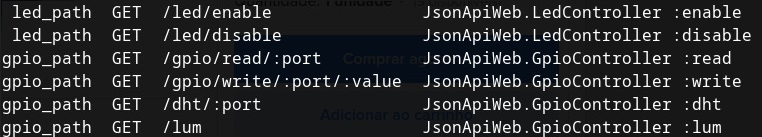
\includegraphics[width=1\textwidth]{assets/static/img/rotas.jpg}
\label{fig:routes}

\begin{minipage}{0.5\textwidth}
\end{minipage}
\end{figure}

\section{Aplicação com Nerves}
O primeiro passo para a utilização do \emph{framework} Nerves em nosso projeto foi realizar o estudo da documentação. Após uma extensa revisão do documento, implementamos um projeto simples que foi sugerido pelo mesmo. Este, consistiu em controlar um led \emph{onboard} do Raspberry pi a partir de uma requisição HTTP.\par
Após consolidação do processo de compilação e entendimento da lógica aplicada nessa aplicação, iniciamos o desenvolvimento do projeto de forma modular e gradativa. Primeiro, começamos com o controle dos GPIOs, em seguida com o sensor de temperatura/umidade e por fim o sensor de luminosidade. Para cada implementação foi necessário localizar e estudar os melhores recurso disponível.\par
Com o desenvolvimento do \emph{firmware} finalizado, partimos para a integração da comunicação entre o \emph{firmware} e o \emph{back-end}, com a finalidade de testar todos os recursos implementados no \emph{firmware}. Após a validação do funcionamento, iniciamos o desenvolvimento do \emph{front-end} para criar uma interface intuitiva e fácil para o usuário.

\begin{figure}[H]
\centering
\caption{Resquisção para a escrita no GPIO 16}
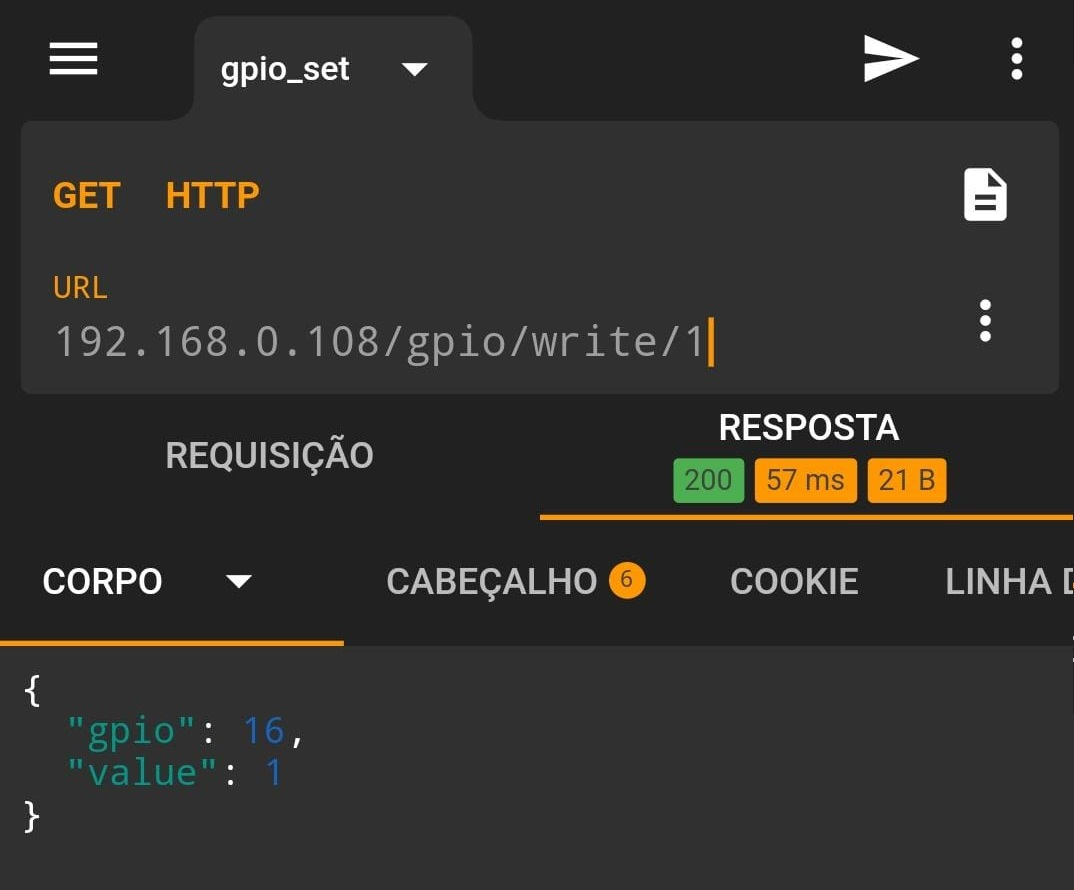
\includegraphics[width=0.5\textwidth]{assets/static/img/request.jpg}
\label{fig:request_gpio}

\begin{minipage}{0.5\textwidth}
\end{minipage}
\end{figure}

\section{Interface de usuário}
A interface do projeto tem como premissa apresentar as informações para o usuário de forma clara e objetiva. Sendo assim, criamos uma interface de tela única baseada em \emph{cards}. O resultado final está apresentado na Figura \ref{fig:ui}.\par
Um \emph{card} representa uma entidade renderizada na tela que tem por objetivo apresentar para o usuário uma informação. Temos três tipos de \emph{cards}:

\begin{enumerate}[label=\alph*)]
\itemsep0em
	\item DHT: exibe as informações fornecidas pelo sensor de temperatura. O botão ``REFRESH'' força a atualização do valor exibido.
	\item Entrada: exibe o estado lógico da entrada escolhida. O botão ``REFRESH'' força a atualização do valor exibido.
	\item Saída: exibe o estado lógico e apresenta opções para ligar e desligar a saída escolhida nos botões ``ON'' e ``OFF''.
\end{enumerate}

\begin{figure}[H]
\centering
\caption{Interface de usuário para controle do hardware}
\includegraphics[width=1\textwidth]{assets/static/img/paralysis.png}
\label{fig:ui}

\begin{minipage}{0.5\textwidth}
\end{minipage}
\end{figure}

O campo ``API URL'' deve ser preenchido com o endereço IP ou DNS do dispositivo na rede, para que possa acontecer a comunicação.

A interface de usuário para controle do hardware foi desenvolvida utilizando um \emph{framework} de \emph{front-end} chamado \emph{React}, que usa uma abordagem modular para a composição de telas.
Dentro do \emph{framework} os módulos que representam as entidades a serem rederizadas na tela são chamados de \emph{componentes}. Os \emph{cards} foram construídos dentro dessa abstração de componentes, assim conseguimos compor eles na tela de forma dinâmica.

\end{document}
